\documentclass[10pt,a4paper]{article}
\usepackage[utf8]{inputenc}
\usepackage{amsmath}
\usepackage{amsfonts}
\usepackage{amssymb}
\usepackage{graphicx}
\usepackage{caption}
\usepackage{subcaption}
\usepackage{float}

\author{Daniel Brown and Dohyun Kim}
\title{Exploration of Different Gradient Ascent Methods for Bayesian Inverse Reinforcement Learning}
\begin{document}
\maketitle

\section{Introduction}
Markov Decision Processes (MDPs) are a commonly used model for sequential decision making tasks. Many different methods including as dynamic programming and temporal difference methods have been proposed to allow a learning agent to solve for the optimal policy of an MDP. However, in some tasks it can be hard to specify a reward function and may be easier to provide demonstrations. This leads to the problem of Inverse Reinforcement Learning (IRL) \cite{ng2000algorithms}. Given an MDP$\setminus$R (an MDP without a specified reward function), and a set of demonstrations consisting of state-action pairs, we wish to recover the reward function that makes the demonstrations optimal. 

Many approaches have been proposed to solve this problem. We choose to focus on the Bayesian IRL setting \cite{ramachandran2007bayesian}. Gradient methods have been proposed to solve this problem \cite{lopes2009active,choi2011map} but contain no details about the specifics of how to perform gradient ascent. We seek to find the MAP estimate of the true reward by maximizing the posterior of the reward $R$ given a set of demonstrations $D$ where
\begin{equation}
P(R | D) \propto P(D | R) P(R)
\end{equation}
The likelihood $P(D|R)$ is defined in a form of softmax function \cite{sutton1998reinforcement} as 
\begin{equation}
P(D | R) = \frac{e^{\alpha \sum_i Q^*(s_i,a_i;R)}}{\sum_{b \in A} e^{\alpha \sum_i Q^*(s_i,b;R)}}
\end{equation}
where $Q^*(s,a; R)$ is the optimal Q-value function for reward $R$ and $\alpha$ is a confidence parameter defining how reliable the demonstrations are. The prior $P(R)$ can be any function. 

We want to use gradient ascent to update to find 
\begin{equation}
R_{MAP} = \arg \max_R  P(R | D) = \arg \max_R [\log(P(D|R) + \log P(R)]
\end{equation}
 reward function to maximize the posterior, thus our update takes the form
\begin{equation}
R_{new} \leftarrow R + \eta_t \nabla_R [\log(P(D|R) + \log P(R)]
\end{equation}

We propose to explore some of the different flavors of gradient ascent we have discussed in class as they apply to the problem of solving the IRL problem.

\section{Gradient Computation}
We first considered just the maximum likelihood estimate of the reward (corresponding to a uniform prior). To perform gradient ascent we need to find the gradient of the likelihood function. We have 
\begin{eqnarray}
\nabla_R \log P(D | R) = \nabla_R \log \prod_{(s,a) \in D} P(a | s, R) \\
=\sum_{(s,a) \in D} \nabla_R \log \frac{e^{\alpha Q_R^*(s,a)}}{\sum_{b \in A} e^{\alpha Q_R^*(s,b)}}\\
= \sum_{(s,a) \in D} \nabla_R \alpha Q_R^*(s,a) - \log \sum_{b \in A} e^{\alpha Q_R^*(s,b)}\\
= \sum_{(s,a) \in D} \alpha \nabla_R Q_R^*(s,a) - \frac{\alpha}{Z_a}\bigg(\sum_{b \in A} e^{\alpha Q_R^*(s,b)} \nabla_R Q_R^*(s,b)\bigg)\\
\end{eqnarray}

where 
\begin{equation}
Z_a = \sum_{b \in A} e^{\alpha Q_R^*(s,b)}
\end{equation}
To compute $\nabla_R Q^*_R(s,u)$ for some action $u$, we note that 
\begin{equation}
V^{\pi} = R + \gamma T^{\pi} V^{\pi}
\end{equation}
so 
\begin{equation}
Q^*_u = R + \gamma T^a V^{\pi^*} = R + \gamma T^a(I - \gamma T^{\pi^*})^{-1}R
\end{equation}
and
\begin{eqnarray}
\frac{\partial Q(s,u)}{\partial R_i} = \delta_i(s) + \gamma W(s,i)
\end{eqnarray}
where $W = T^a(I - \gamma T^{\pi^*})^{-1}$

\section{Approach}
We investigated a simple, yet scalable navigation domain where a subset of states have negative reward (obstacles) most states have zero reward and the goal state has positive reward. Given a few demonstration trajectories, we wish to recover the reward using gradient ascent. We implemented gradient ascent and evaluated different step sizes. We also considered how to recover a sparse reward by adding a regularization term and using subgradients. We showed that our methods work well, but at a large computation cost. We finally investigated stochastic gradient ascent, but found that a large part of our computation cost was due to computing the Q-values by solving the underlying MDP, thus limiting the number of demonstrations reduces some of the cost, but not enough to make it worthwhile. 

\section{Results}

\subsection{Gradient ascent with various step sizes}
Our first result is the tendency of the objective function, log-likelihood posterior probability, with different step sizes. We have considered three kinds of step sizes namely constant, decreasing with speed proportional to $1/\sqrt{t}$ and $1/t$ where $t$ is the number of iterations performed. Since the function is a form of softmax, which is a normalized exponential distribution, our expectations were that the Gradient ascent will minimize the policy difference $\| \pi - \pi^{*} \|$. The results are shown in Figure~\ref{fig:step_size}.

\begin{figure}
    \centering
    \begin{subfigure}[b]{0.65\textwidth}
        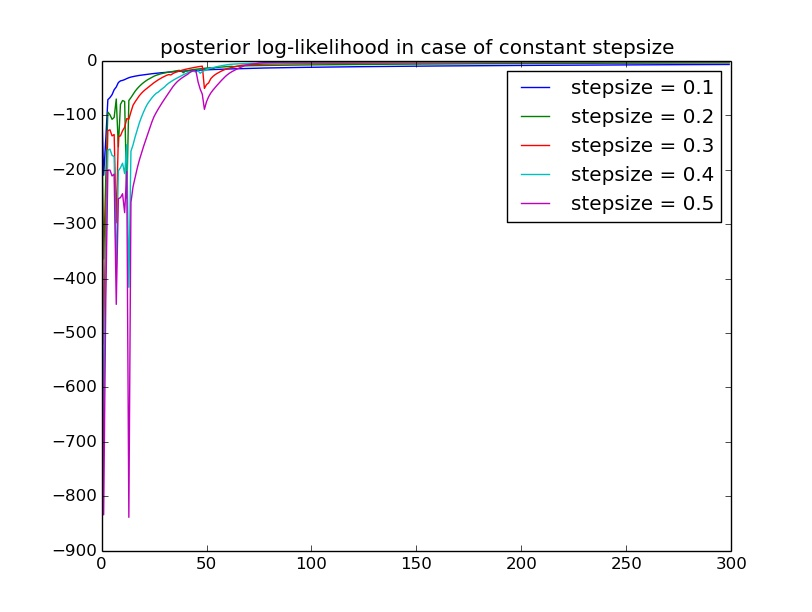
\includegraphics[width=\textwidth]{figs/constant_stepsize.jpg}
        \caption{Gradient ascent performed with constant stepsize}
    \end{subfigure}
    ~ %add desired spacing between images, e. g. ~, \quad, \qquad, \hfill etc. 
      %(or a blank line to force the subfigure onto a new line)
    \begin{subfigure}[b]{0.65\textwidth}
        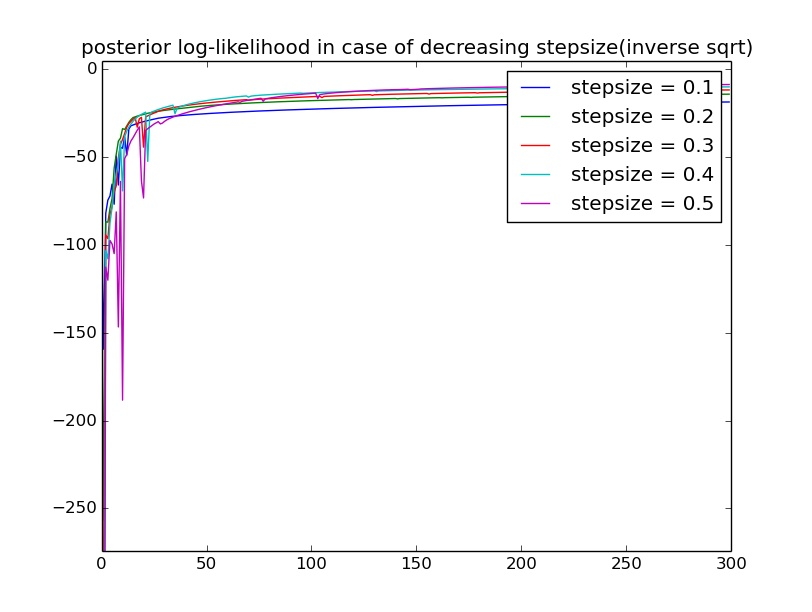
\includegraphics[width=\textwidth]{figs/decreasing_stepsize_inv(sqrt).jpg}
        \caption{Gradient ascent performed with decreasing stepsize(inverse sqrt)}
    \end{subfigure}
    \begin{subfigure}[b]{0.65\textwidth}
        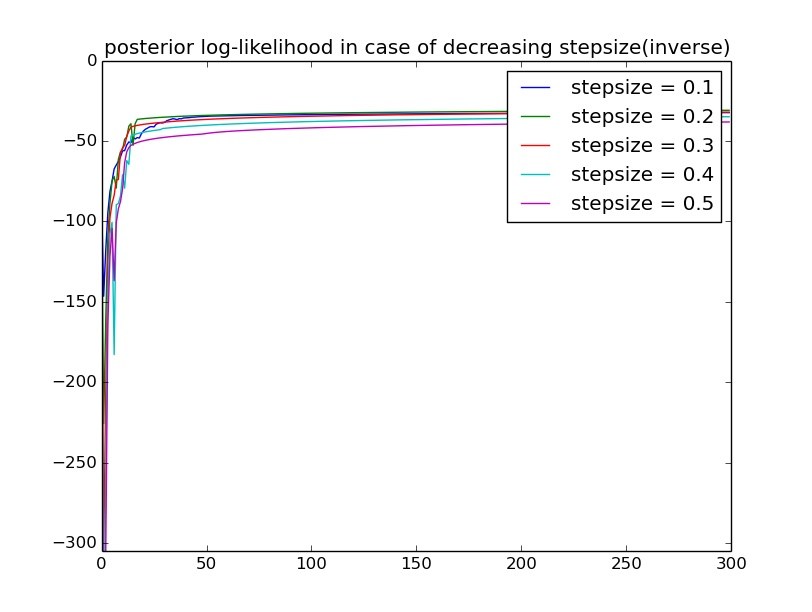
\includegraphics[width=\textwidth]{figs/decreasing_stepsize_inv(linear).jpg}
        \caption{Gradient ascent performed with decreasing stepsize(inverse linear)}
    \end{subfigure}
    \caption{Gradient ascent performed with various step sizes}
    \label{fig:step_size}
\end{figure}

Within a step size category, constant coefficients 0.1, 0.2, 0.3, 0.4 and 0.5 were used for comparison. The results show that all three kinds of step sizes can be used to perform gradient ascent as they all converge to the optimal point. In this case, the optimal point is respect to the policy difference  $\| \pi - \pi^{*} \|$ meaning $\| \pi - \pi^{*} \| = 0$ at the optimal point. 

\begin{figure}
    \centering
        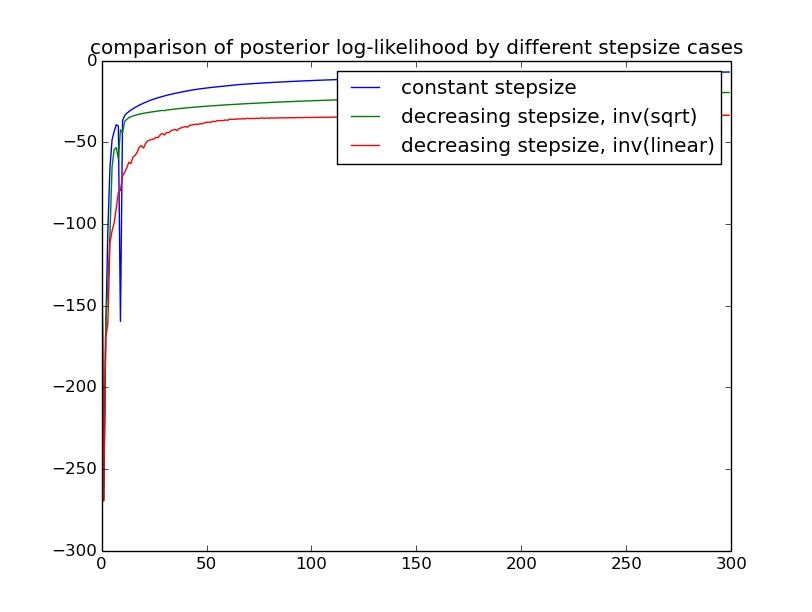
\includegraphics[width=0.55\textwidth]{figs/comparison_stepsize.jpg}
        \caption{Comparison of Gradient ascent performed with different stepsize}
        \label{fig:step_comparison}
\end{figure}

Comparing the three kinds of stepsizes(constant, inverse sqrt and inverse), we have used $c=0.1$. The plot in Figure~\ref{fig:step_comparison} shows that for constant coefficient $c=0.1$, gradient ascent with inverse sqrt step size converges faster than the other two and constant step size shows the most slow convergence. Although the objective function value shows that the gradient ascent with constant step size has the maximum, the "hidden" objective function is the policy difference and gradient ascent with inverse sqrt step size has the best performance.


\subsection{Recovering a sparse reward}
We noticed that even though gradient ascent usually recovers the optimal policy, the reward it finds is rarely sparse. However, in many sequential decision making tasks the reward is sparse. To try to better recover the expert's true reward when the reward is known to be sparse we added an $L^1$-norm regularization. Our new objective function is 
\begin{equation}
\max_R \log P(D|R) - \lambda \|R\|_1
\end{equation}

To test this method out we designed a simple $4\times 7$ grid navigation task where there is a winding path of smooth ground where travel costs are zero and patches of rough ground where travel costs are -1, there is also a terminal goal state with a reward of +1 in the top left corner. The true reward is shown in Figure~\ref{subfig:true_sparse_reward}. We optimized the regularized objective using subgradient ascent for different values of the regularization parameter $\lambda$.

\begin{figure}
    \centering
    \begin{subfigure}[b]{0.55\textwidth}
        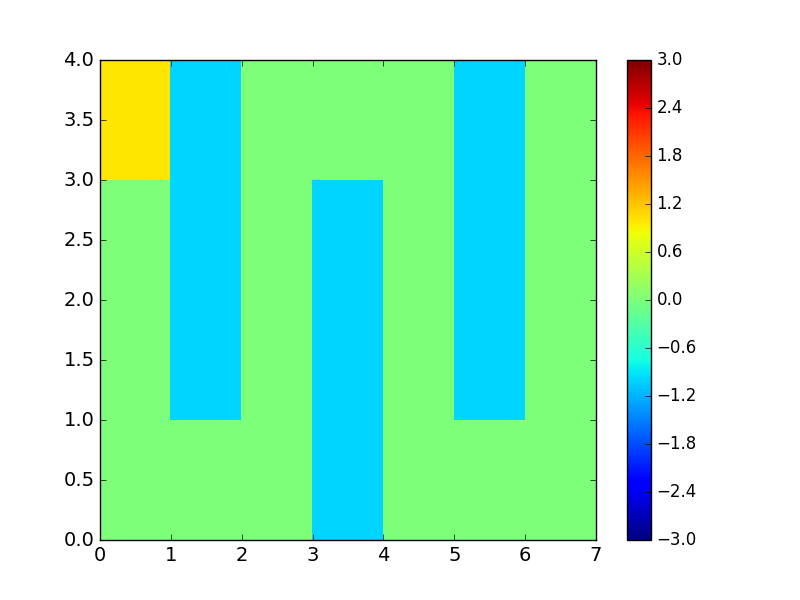
\includegraphics[width=\textwidth]{figs/true_reward.png}
        \caption{True sparse reward used by demonstrator}
        \label{subfig:true_sparse_reward}
    \end{subfigure}
    ~ %add desired spacing between images, e. g. ~, \quad, \qquad, \hfill etc. 
      %(or a blank line to force the subfigure onto a new line)
    \begin{subfigure}[b]{0.55\textwidth}
        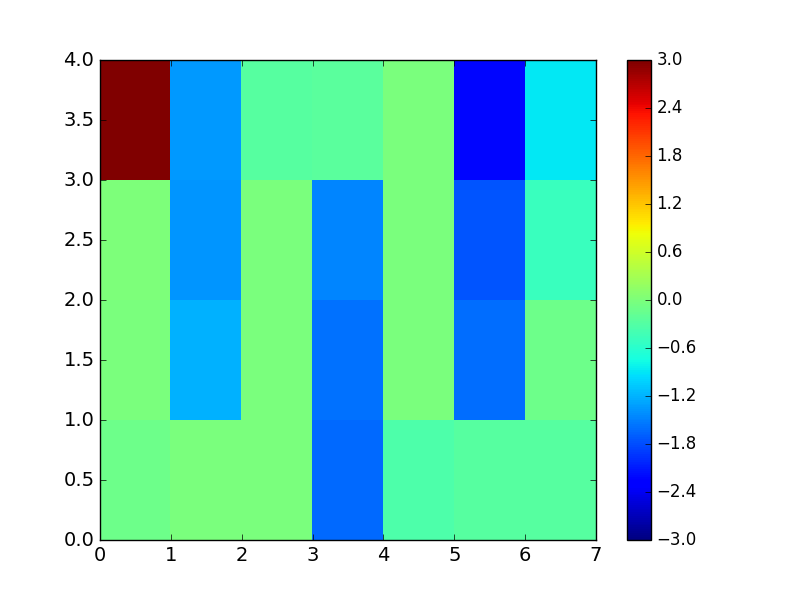
\includegraphics[width=\textwidth]{figs/recovered_reward_lam0_5.png}
        \caption{Recovered reward using regularization with $\lambda = 0.5$}
        \label{subfig:recovered_sparse_reward}
    \end{subfigure}
    \caption{True and recovered sparse reward. Sparse reward is learned using subgradient ascent.}\label{fig:sparse_reward}
\end{figure}

Figure~\ref{fig:regularization_test} shows the results. We see if Figure~\ref{subfig:reg_L1-norm} that, as expected, higher regularization results in lower $L^1$-norm of the learned reward. We also see in Figure~\ref{subfig:reg_reward_diff} that using a larger regularization term results in a recovered reward that is much closer to that of the experts. Figure~\ref{subfig:reg_policy_diff} shows that too much regularization ($\lambda = 1.0$) causes the algorithm to find a sparse reward that does not result in a good policy, while a regularization term of $\lambda = 0.5$ seems to do best in terms of recovering a sparse reward that still induces a policy that matches the expert. We have plotted a heatmap of the learned reward when $\lambda=0.5$ in Figure~\ref{subfig:recovered_sparse_reward}. The regularization helps the algorithm to find a reward that is close to zero along the path and has non-zero rewards at the goal and along the rougher terrain.

 Interestingly, the tests run with smaller regularization terms immediately found rewards that produced the expert's policy, which is why the lines are not visible in Figure~\ref{subfig:reg_policy_diff}; however, using these smaller regularization terms resulted in a type of reward overfitting, where non-sparse rewards were learned to try to maximize the likelihood of the demonstrations.


\begin{figure}
    \centering
    \begin{subfigure}[b]{0.65\textwidth}
        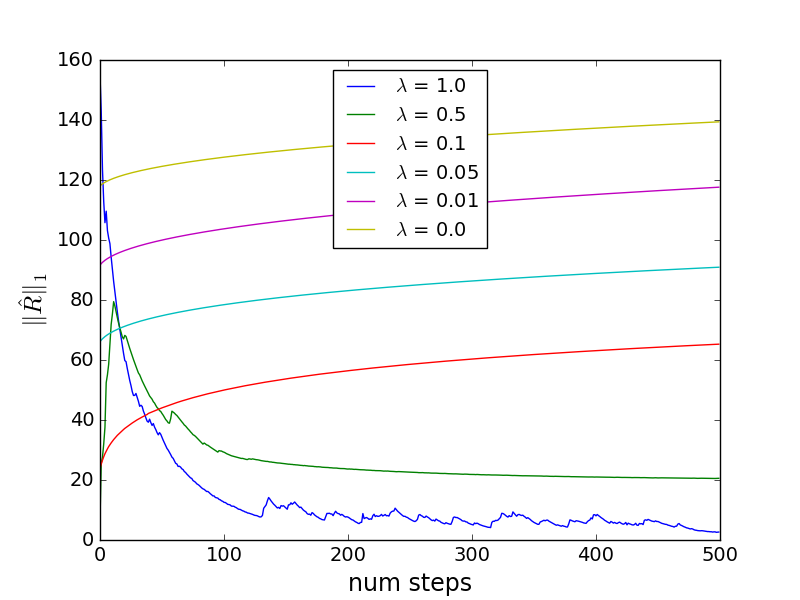
\includegraphics[width=\textwidth]{figs/reward_norm_reg_test.png}
        \caption{$L^1$-norm of learned reward function.}
        \label{subfig:reg_L1-norm}
    \end{subfigure}
    \begin{subfigure}[b]{0.65\textwidth}
        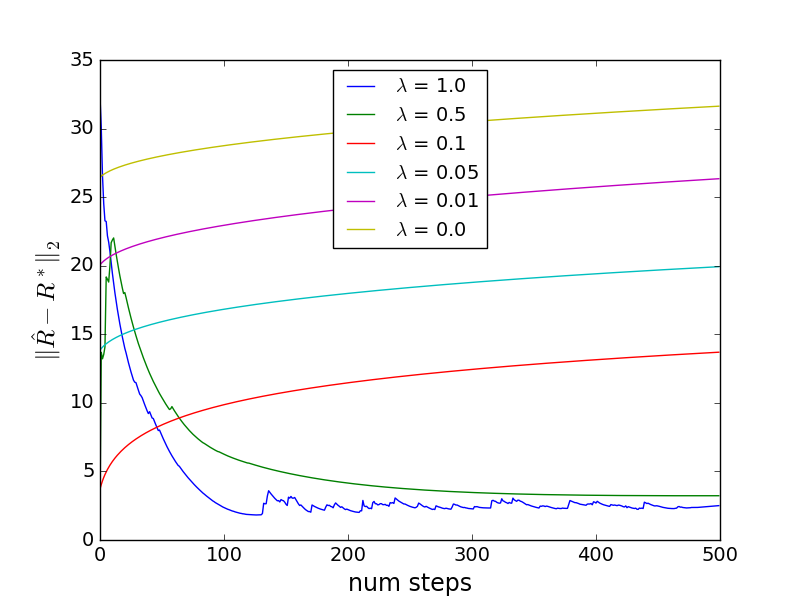
\includegraphics[width=\textwidth]{figs/reward_diff_reg_test.png}
        \caption{Error between true reward and recovered reward.}
        \label{subfig:reg_reward_diff}
    \end{subfigure}
    ~ %add desired spacing between images, e. g. ~, \quad, \qquad, \hfill etc. 
      %(or a blank line to force the subfigure onto a new line)
    
    \begin{subfigure}[b]{0.65\textwidth}
        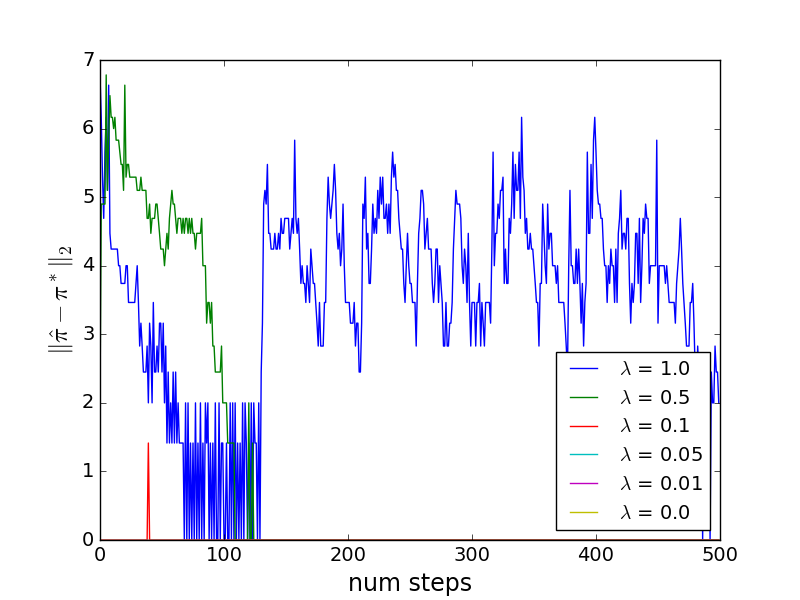
\includegraphics[width=\textwidth]{figs/policy_diff_reg_test.png}
        \caption{Difference between expert policy and learned policy.}
        \label{subfig:reg_policy_diff}
    \end{subfigure}
    \caption{Evaluation of subgradient ascent for different regularization parameters as a function of number of steps.}\label{fig:regularization_test}
\end{figure}

Our results show adding regularization is a way to recover a sparse reward from expert demonstrations. This could be useful in cases where it is known that the domain has only sparse rewards, as well as in general cases as a type of Occam's razor that prefers simpler (sparse) rewards to explain an expert's behavior.

\subsection{Run-time analysis}
We examined the run-term per gradient calculation and found it to be quite high for larger numbers of states. However, this is to be expected since there is an inverse involved in the gradient computation in order to solve the MDP with the current reward guess. The run-time results are shown in Figure~\ref{fig:run_time_gd}

\begin{figure}
\centering
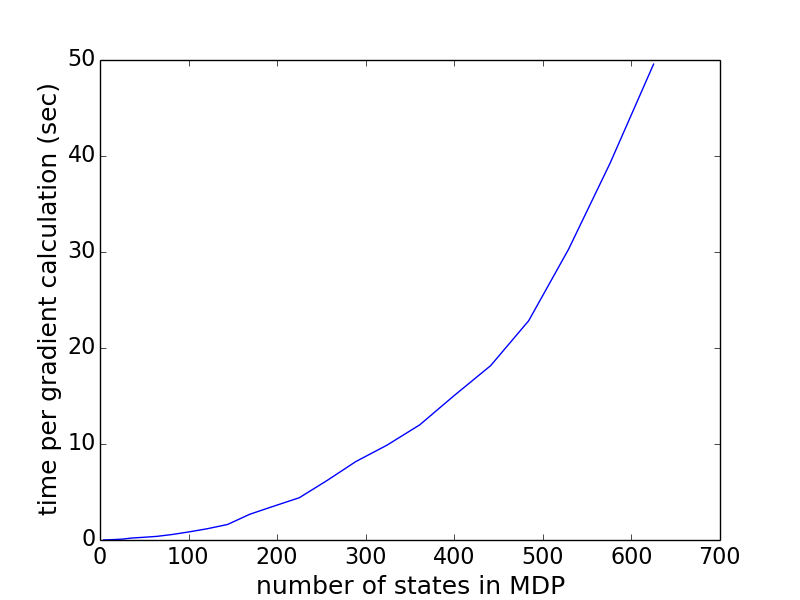
\includegraphics[scale=0.4]{figs/ave_run_time.png}
\caption{Average time to compute a single gradient step }
\label{fig:run_time_gd}
\end{figure}

\subsection{Stochastic Gradient Ascent}
We had initially hoped to use Stochastic Gradient Ascent to try to reduce the computation cost of computing the gradient. As derived above, the gradient is of the form 
\begin{eqnarray}
\nabla_R \log P(D | R) = \sum_{(s,a) \in D} \bigg(\alpha \nabla_R Q_R^*(s,a) - \frac{\alpha}{Z_a}\bigg(\sum_{b \in A} e^{\alpha Q_R^*(s,b)} \nabla_R Q_R^*(s,b)\bigg) \bigg).
\end{eqnarray}
At first glance, this appears to be amenable to stochastic gradient ascent, since the gradient is a sum of gradients with respect to each state-action pair in the demonstration $D$. However, there is an implicit coupling because of the need to compute the optimal Q-values to compute the gradient for each term in the summation. This requires solving an MDP, which is where the brunt of the computation lies. Thus, if we are going to go through the trouble of calculating the Q-values in order to calculate the gradient with respect to one state-action pair, we should reuse this computation and compute the full gradient rather than repeatedly taking a step for a single state-action pair which would require repeatedly solving for the Q-values after every mini-batch, giving us a noisier gradient step at a nearly identical cost to the full gradient step.

To test this intuition we ran an experiment on a 25x25 grid where we computed the average time to compute a single gradient step when given 1,50,100, and 200 demonstrations. The average run times in seconds are shown in Table~\ref{tab:run_time_sgd}. These results show that a lot of the computation time is due to the need to solve the MDP, but that in cases with large numbers of demonstrations, taking the gradient with respect to a random subset may alleviate some of the computational burden and might result in improved run-times. We tried several experiments with different step sizes and mini-batch sizes, but could not find any improvement using stochastic gradient ascent.

\begin{table}
\centering
\begin{tabular}{|c|c|c|c|c|c|}
\hline 
num (s,a) pairs & 1 & 50 & 100 & 200 & 600\\ 
\hline
run-time (sec) & 11.92 & 12.65 & 12.87 & 14.79 & 20.5 \\ 
\hline 
\end{tabular}
\caption{Average time to compute one gradient step for different numbers of (s,a) pairs given as demonstration for a grid world of size 25x25.}
\label{tab:run_time_sgd}
\end{table}


\section{Discussion and Future Work}
Our results for varying step sizes showed that using a constant step size with constant coefficient 0.1 had the least amount of oscillation, but the convergence speed for larger step sizes was slightly faster. We also compared inverse square root and inverse decreasing step sizes. We found that using a constant step size achieved the highest log likelihood, but suffered from some oscillations. The inverse square root step size quickly converged, but to a slightly worse objective value. The inverse step size also converged to a worse objective value. Despite having different log likelihoods, the policies learned using the different step sizes all converged to the expert's policy. We hypothesize that this is because the objective function is not smooth---due to the fact that small changes in reward can cause large changes in the optimal policy---and because many rewards can lead to the same optimal policy. Thus the decreasing step sizes led to slightly worse local optima in terms of the objective but still recovered the correct policy.

We also investigated how to recover a reward that is known to be sparse. We found that standard gradient ascent typically found a non-zero reward function. However, by adding an $L^1$-norm regularization term we were able to recover rewards that were sparse and much closer to the true reward. This could be beneficial in cases where an agent needs to learn from demonstrations in one MDP and then transfer its learned reward to a new MDP. Regularization helps the algorithm avoid overfitting to a single domain and instead provides a type of Occam's razor that seeks a simple reward to explain the observed behavior. This would be beneficial in applications where the motivations behind the demonstrations are important.

Finally, we investigated the run-time of our algorithm. We found that computing a single gradient step can be very costly since it involves fully solving an MDP. Despite the apparent separability of the objective function over state-action pairs, solving the MDP is required for every step so we were unable to get significant benefits from stochastic gradient ascent. Future work should investigate IRL methods that avoid solving an MDP at each iteration. Future work should also investigate methods to speed up convergence such as backtracking line search or accelerated methods. We experimented with backtracking line search, but we were unable to get it work, possibly due to smoothness issues in the objective function.


\bibliographystyle{plain}
\bibliography{proposal.bib}


\end{document}